% Generated by code/scripts/report_figures.py at 2026-11-03T07:57:50Z; do not edit.
% Inputs: artifacts/local/runs/pipeline-e2e-20261103T075711Z/run
\begin{figure}[t]
\centering
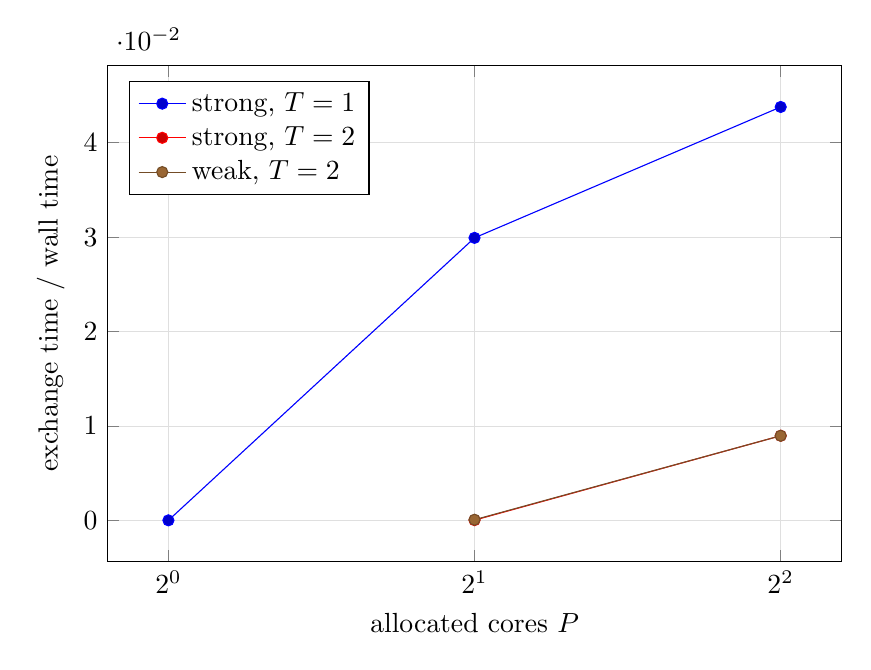
\begin{tikzpicture}
\begin{axis}[width=0.9\columnwidth, height=0.65\columnwidth, xlabel={allocated cores $P$}, ylabel={exchange time / wall time}, xmode=log, log basis x=2, legend pos=north west, legend cell align=left, grid=major, grid style={gray!25}]
\addplot+[mark=*] coordinates {(1,1.762e-05) (2,0.02993) (4,0.04379)};
\addlegendentry{strong, $T=1$}
\addplot+[mark=*] coordinates {(2,3.559e-05) (4,0.008975)};
\addlegendentry{strong, $T=2$}
\addplot+[mark=*] coordinates {(2,8.277e-05) (4,0.008975)};
\addlegendentry{weak, $T=2$}
\end{axis}
\end{tikzpicture}
\caption{\textbf{LOCAL PIPELINE TEST, NOT A MEASUREMENT.} Share of the timed region spent in the per-step position exchange (\texttt{MPI\_Allgatherv}), maximum over ranks divided by wall time.}
\label{fig:comm-fraction}
\end{figure}
